\documentclass[12pt, oneside]{report}

\usepackage[utf8]{inputenc} % Required for inputting international characters
\usepackage[T1]{fontenc} % Output font encoding for international characters
\usepackage[a4paper,left=1in,right=1in,top=.75in,bottom=.75in]{geometry}
\usepackage{mathpazo} % Palatino font
\usepackage{graphicx}
\usepackage{sectsty}
\usepackage{epigraph}
\usepackage{indentfirst}
\usepackage{float}
\usepackage[pagestyles]{titlesec}
\usepackage{setspace}
\usepackage[nottoc,notlof,notlot]{tocbibind}

% \renewcommand{\baselinestretch}{1.5} 

\renewcommand\bibname{References}
\titleformat{\chapter}[display]
{\normalfont\Large\bfseries}{\scshape\chaptertitlename\ \thechapter}{20pt}{\filcenter\LARGE\scshape}


\titlespacing*{\chapter}{0pt}{0pt}{20pt}
\titleformat*{\section}{\Large\bfseries}
\titleformat*{\subsection}{\large\bfseries}
\setlength\epigraphwidth{.8\textwidth}
\setlength\epigraphrule{1pt}


\renewpagestyle{plain}{
  \setheadrule{.4pt}
  \setfootrule{.4pt}% Header rule
  \setfootrule{.4pt}% Footer rule
  \sethead[Image Regeneration with Generative Models]% odd-left
          []% odd-center
          [\chaptertitle]% odd-right
          {Image Regeneration with Generative Models}% even-left
          {}% even-center
          {\chaptertitle}% even-right
  \setfoot[Dept. of CSE, Sir MVIT]% odd-left
          []% odd-center
          [\thepage]% odd-right
          {Dept. of CSE, Sir MVIT}% even-left
          {}% even-center
          {\thepage}% even-right
}

\pagestyle{plain}


\begin{document}

%----------------------------------------------------------------------------------------
{\setstretch{1.0}

%----------------------------------------------------------------------------------------
%	TITLE PAGE
%----------------------------------------------------------------------------------------

\begin{titlepage} % Suppresses displaying the page number on the title page and the subsequent page counts as page 1
	\newcommand{\HRule}{\rule{\linewidth}{0.5mm}} % Defines a new command for horizontal lines, change thickness here

	\center % Centre everything on the page

	%------------------------------------------------
	%	Headings
	%------------------------------------------------
	\textsc{\LARGE Visvesvaraya Technological University\\[3pt]Belgaum 590014}\\[10pt] 
	%------------------------------------------------
	%	Logo
	%------------------------------------------------
	
\includegraphics[width=0.15\textwidth]{images/vtu.png}\\[10pt] 

	{\Large Synopsis Entitled}\\[10pt] % Major heading such as course name

	%------------------------------------------------
	%	Title
	%------------------------------------------------

	\HRule\\[10pt]
	\textsc{\huge \textbf{Image Regeneration With Generative}\\[3pt] \textbf{Models}}\\[10pt]

	\HRule\\[10pt]
	\Large{
		Submitted for\\
		\textbf{Bachelor Of Engineering}\\
		In \\
		\textbf{Computer Science And Engineering} \\
		For the Academic year 2017-2018 
	}\\[15pt]
	\Large{Submitted by}\\[2pt]
	%------------------------------------------------
	%	Author(s)
	%------------------------------------------------
	\begin{tabular}{ l r }
		\textsc{\Large \textbf{Abhijith C.}}       & \Large \textbf{1MV14CS004} \\
		\textsc{\Large \textbf{Raghava G. Dhanya}} & \Large \textbf{1MV14CS077} \\
		\textsc{\Large \textbf{Shashank S.}}       & \Large \textbf{1MV14CS131}
	\end{tabular}\\[15pt]

	\Large{Project carried out at\\
		\textbf{Sir M. Visvesvaraya Institute of Technology}
		\\Bangalore-562157
	}\\[10pt]
	\Large{Under the Guidance of\\
		\textbf{\textsc{\Large Mrs. Sushila Shidnal }}\\
		Assistant Professor, Department of CSE\\
		Sir M Vivesvaraya Institute of Technology, Bangalore.
	}\\[10pt]
	%------------------------------------------------
	%	Logo
	%------------------------------------------------
	
\includegraphics[width=0.15\textwidth]{images/mvit.png}\\[10pt] 
	\Large{
		\textbf{Department Of Computer Science \& Engineering}\\
		\textbf{Sir M. Visvesvaraya Institute Of Technology}\\
		Hunasamaranahalli, Bangalore-56215\\
	}

\end{titlepage}

\par

%----------------------------------------------------------------------------------------
%	TITLE PAGE
%----------------------------------------------------------------------------------------

\begin{titlepage} % Suppresses displaying the page number on the title page and the subsequent page counts as page 1
	\newcommand{\HRule}{\rule{\linewidth}{0.5mm}} % Defines a new command for horizontal lines, change thickness here

	\center % Centre everything on the page

	%------------------------------------------------
	%	Headings
	%------------------------------------------------
	\textsc{\LARGE Visvesvaraya Technological University\\[3pt]Belgaum 590014}\\[10pt] 
	%------------------------------------------------
	%	Logo
	%------------------------------------------------
	
\includegraphics[width=0.15\textwidth]{images/vtu.png}\\[10pt] 

	{\Large Synopsis Entitled}\\[10pt] % Major heading such as course name

	%------------------------------------------------
	%	Title
	%------------------------------------------------

	\HRule\\[10pt]
	\textsc{\huge \textbf{Image Regeneration With Generative}\\[3pt] \textbf{Models}}\\[10pt]

	\HRule\\[10pt]
	\Large{
		Submitted for\\
		\textbf{Bachelor Of Engineering}\\
		In \\
		\textbf{Computer Science And Engineering} \\
		For the Academic year 2017-2018 
	}\\[15pt]
	\Large{Submitted by}\\[2pt]
	%------------------------------------------------
	%	Author(s)
	%------------------------------------------------
	\begin{tabular}{ l r }
		\textsc{\Large \textbf{Abhijith C.}}       & \Large \textbf{1MV14CS004} \\
		\textsc{\Large \textbf{Raghava G. Dhanya}} & \Large \textbf{1MV14CS077} \\
		\textsc{\Large \textbf{Shashank S.}}       & \Large \textbf{1MV14CS131}
	\end{tabular}\\[15pt]

	\Large{Project carried out at\\
		\textbf{Sir M. Visvesvaraya Institute of Technology}
		\\Bangalore-562157
	}\\[10pt]
	\Large{Under the Guidance of\\
		\textbf{\textsc{\Large Mrs. Sushila Shidnal }}\\
		Assistant Professor, Department of CSE\\
		Sir M Vivesvaraya Institute of Technology, Bangalore.
	}\\[10pt]
	%------------------------------------------------
	%	Logo
	%------------------------------------------------
	
\includegraphics[width=0.15\textwidth]{images/mvit.png}\\[10pt] 
	\Large{
		\textbf{Department Of Computer Science \& Engineering}\\
		\textbf{Sir M. Visvesvaraya Institute Of Technology}\\
		Hunasamaranahalli, Bangalore-56215\\
	}

\end{titlepage}

\par
}
\pagenumbering{roman}
\begin{titlepage}
\begin{center}
\noindent\textsc{\textbf{\Large Sir M Visvesvaraya Institute of Technology}}\\[3pt]
\textsc{\textbf{\large Bengaluru 562157\\[3pt]Department of Computer Science and Engineering}}\\[15pt]

\includegraphics[width=0.2\textwidth]{images/mvit.png}\\[15pt] 
\textsc{\textbf{\Large Certificate}}\\
\end{center}
This is to certify that the project work entitled "Image Regeneration With Generative Models" has been carried out by Abhijith C. (1MV14CS004), Raghava G. Dhanya (1MV14CS077) and Shashank S. (1MV14CS131), bona-fide students of Sir M Visvesvaraya Institute of Technology, in partial fulfillment for the award of the Degree of Bachelor of Engineering in Computer Science and Engineering of the Visvesvaraya Technological University, Belagavi during the year 2016-2017. It is certified that all corrections and suggestions indicated during Internal Assessment have been incorporated into the report deposited in the department library. The project report has been approved as it satisfies the academic requirements with respect to the project work prescribed for the course of Bachelor of Engineering.

\vspace{100px}

\noindent
\begin{tabular*}{\textwidth}{@{} l @{\extracolsep{\fill}} l @{\extracolsep{\fill}} l @{}}
    \textsc{\textbf{\small Mrs. Sushila Shidnal}} & \textsc{\textbf{\small Prof. Dilip K Sen}}  & \textsc{\small \textbf{Dr. V. R. Manjunath}}\\
    \textbf{\small Asst. Prof \& Internal Guide}   & \textbf{\small Head of Department} & \textbf{\small Principal}\\
    \textbf{\small Dept. of CSE, Sir MVIT}        & \textbf{\small Dept. of CSE, Sir MVIT}           &  \textbf{\small Sir MVIT}
\end{tabular*}\\[35pt]
\textbf{Name of the examiners}\hfill\textbf{Signature with date}\\
1)\\
2)
\end{titlepage}\par
\chapter*{Abstract\markboth{Abstract}{Abstract}}\label{ch:abstract}
\addcontentsline{toc}{chapter}{Abstract}

Current advances in Generative Adversial Networks allow us to obtain near realistic images of faces but it is still quite distinguishable from actual photographic images. The technology is also not very amiable to changes in the orientation of faces in Convolutional Neural Networks(CNN). Additionally, the amount of data required to train the network must be exhaustible, for example, in case different perspectives of a face are required the various perspectives must be explicitly present in the training data to achieve the result. Thus the network requires humongous amounts of data.
\par\bigskip
In this paper we propose a novel approach to accomplish the same results using CapsNet. CapsNet employs a dynamic routing algorithm which replaces the scalar-output feature detectors of the CNN with vector-output capsules. A capsule is essentially a group of neurons describing a specific part of obect or image. Active capsules at one level make predictions, via transformation matrices, for the instantiation parameters of
higher-level capsules. In essence, the CapsNet is the reverse of the common Computer Graphics pipeline where we convert objects to their renders. The CapsNet works from the pixel level and works up towards the object.
\par\bigskip
We propose that the amount of data required to train a comparable model is very small while it gives comparable, if not better, results. \par
\tableofcontents
% \listoffigures
\clearpage
\pagenumbering{arabic}
% \pagestyle{plain}
\chapter{Introduction}\label{ch:introduction}

\epigraph{\textit{\Large "What I cannot create, I do not understand."}}{\textit{ \Large Richard Feynman}}
One of the main aspirations of Artificial Intelligence is to develop algorithms and techniques that enrich computers with ability to understand our world. Generative models are one of the most promising approaches towards achieving this goal.\par\bigskip
A generative model is a mathematical or statistical model to generate all values of a phenomena. To train such a model, we first collect a large amount of data in some domain (e.g., think millions of images, sentences, or sounds, etc.) and then train a model to generate data like it.\par\bigskip
A generative algorithm models how data was generated to classify a signal. It poses the question: according to my generation hypotheses, which category is most likely to generate this signal? A discriminant algorithm does not care about how the data was generated, it just classifies a given signal. A generative model learns the joint probability distribution $p(x,y)$ while a discriminative model learns the conditional probability distribution $p(y|x)$ “probability of y given x”.\par\bigskip
The trick is that the neural networks that we use as generating models have a significantly smaller number of parameters than the amount of data on which we train them, so the models are forced to effectively discover and internalize the essence of the data to generate it.\par\bigskip
There are multiple approaches to build a generative models
\begin{itemize}
  \item Generative adversarial networks (GANs) are a class of generative algorithms used in unsupervised machine learning, implemented by a system of two neural networks competing in a zero-sum game framework. They were presented by Ian Goodfellow et al. in 2014 [1]. This technique can generate photographs that seem at least superficially authentic to human observers, having many realistic features (though in tests people can tell real from generated in many cases).
  \item Variational Autoencoders (VAEs) allow us to formalize this problem in the framework of probabilistic graphical models where we are maximizing a lower bound on the log likelihood of the data
  \item Autoregressive models such as PixelRNN, on the other hand train a network that models the conditional distribution of every individual pixel given previous pixels (to the left and to the top). This is similar to plugging the pixels of the image into a char-rnn, but the RNNs runs both horizontally and vertically over the image instead of just a 1D sequence of characters.
\end{itemize} \par
Generative Adversarial Networks, which we already discussed above, pose the training process as a game between two distinct networks: a generator network (as seen above) and a second discriminative network that tries to classify samples as either coming from the true distribution $p(x)$ or the model distribution $\hat{p}(x)$. Every time the discriminator notices a difference between the two distributions the generator adjusts its parameters slightly to make it go away, until at the end (in theory) the generator exactly reproduces the true data distribution and the discriminator is guessing at random, unable to find a difference.

% \section{Some section}
% blah blah blah
% \subsection{some subsection}
% blah blah
\par
\chapter{Literature Survey}\label{ch:literature_survey}
\epigraph{\textit{\Large “Adversarial training is the coolest thing since sliced bread”}}{\textit{ \large Yann LeCun,\\ Director of AI Research at Facebook and Professor at NYU}}
GANs were first introduced by Ian Goodfellow et al. in 2014[1] in Neural Information Processing Systems 2014 (NIPS 2014). The paper proposes a completely new framework for estimating generative models via an adversarial process. In this process two models are simultaneously trained. According to [1] the network has a generative model G that captures the data distribution, and a discriminative model D that estimates the probability that a sample came from the training data rather than G. This framework corresponds to a minimax two-player game. There is no need for any Markov chains or unrolled approximate inference networks during either training or generation of samples. This original work by Ian Goodfellow uses fully connected neural networks in the generator and the discriminator.\par\bigskip
\begin{figure}[H]
\centering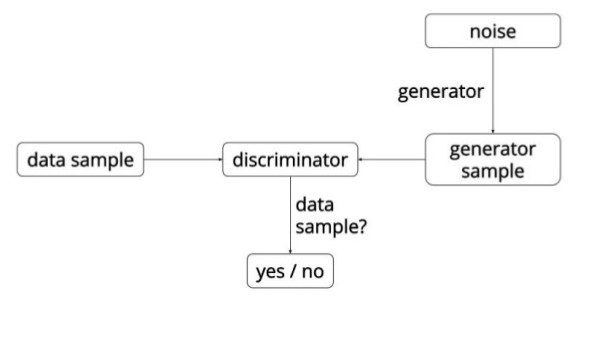
\includegraphics[width=.7\textwidth]{images/vanilaGAN.jpg}
\caption{Vanilla Generative Adversarial Network}
\end{figure}
Since then, there has been tremendous advancements in Deep Learning. A convolutional neural network (CNN, or ConvNet) [2] is a class of deep, feed-forward artificial neural networks that has successfully been applied to analyzing visual imagery. These networks uses convolution layers in its core. The convolution layer's parameters consist of a set of learnable filters, also called as kernels, which have a small receptive field, but they extend through the full depth of the input volume. During the forward pass, each filter is convolved across the width and height of the input volume, computing the dot product between the entries of the filter and the input and producing a 2-dimensional activation map of that filter. As a result, the network learns filters that activate when it detects some specific type of feature at some spatial position in the input.\par\bigskip
\begin{figure}[H]
\centering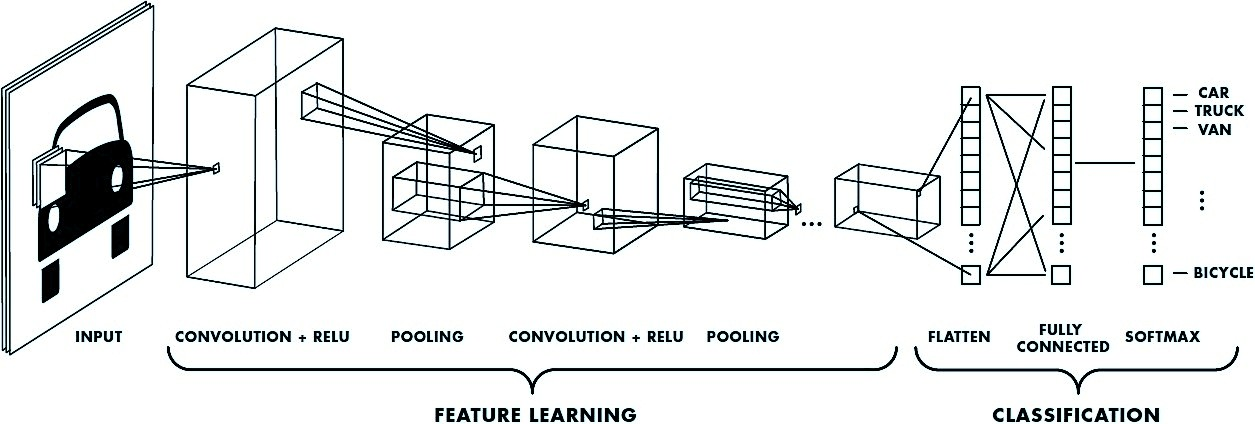
\includegraphics[width=.7\textwidth]{images/CNN.jpg}
\caption{Convolutional Neural Network}
\end{figure}
A breakthrough development that occurred in Adversarial Networks was the introduction of “Deep Convolutional Generative Adversarial Networks” by Alec Radford et al, ICLR, 2016 in 2016 in ICLR[3]. He applied a list of empirically validated tricks as the substitution of pooling and fully connected layers with convolutional layers.\par\bigskip
\begin{figure}[H]
\centering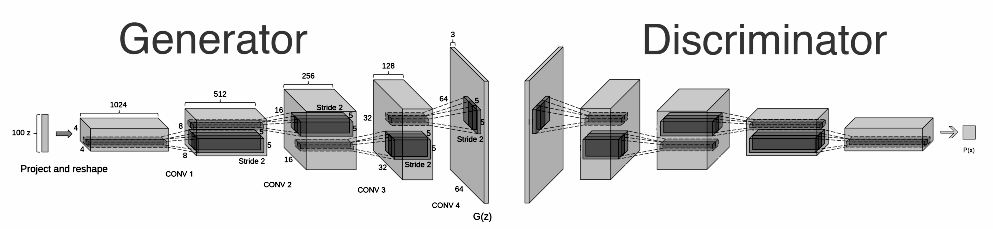
\includegraphics[width=1\textwidth]{images/dcgan.png}
\caption{Deep Convolutional Generative Adversarial Network}
\end{figure}
The power of the features encoded in the latent variables was further explored by Chen at al. [4]. They made use of the fact that the latent space of a regular GAN is underspecified to add additional input parameters (referred to as extend code) and thereby functionality. They decomposed the code in the latent code seen before and an additional latent component, which targets the semantic features of the data distribution. The goal is to learn disentangled and interpretable representations.\par\bigskip
Today, most GANs are loosely based on the former shown DCGAN [3] architecture. Many papers have focused on improving the setup to enhance stability and performance. Many key insights was given by Salimans et al.[5]:
\begin{itemize}
\item Usage of convolution with stride instead of pooling
\item Usage of Virtual Batch Normalization
\item Usage of Minibatch Discrimination in DD
\item Replacement of Stochastic Gradient Descent with Adam Optimizer [6]
\item Usage of one-sided label smoothing
\end{itemize}
Another huge development came with the introduction of Wasserstein GANs by Martin Arjovsky [7] . He introduced a new algorithm named WGAN, an alternative to traditional GAN training. In this new model, he showed that the stability of learning can be improved, remove problems like mode collapse, and provide good learning curves useful for debugging and hyperparameter searches.\par\bigskip
This recently proposed Wasserstein GAN (WGAN) makes progress toward stable training of GANs, but sometimes can still generate only low-quality images or fail to converge. 
Ishaan Gulrajani with Martin Arjovsky proposed an alternative in [8] to fix the issues the previous GAN faced. This proposed method performs better than standard WGAN and enables stable training of a wide variety of GAN architectures with almost no hyperparameter tuning, including 101-layer ResNets[9] and language models over discrete data.\par\bigskip
A big breakthrough in the field of Deep Learning came with the introduction of CapsNets or Capsule Networks[10] by the Godfather of Deep Learning, Geoffrey Hinton. CNNs perform exceptionally great when they are classifying images which are very close to the data set. If the images have rotation, tilt or any other different orientation then CNNs have poor performance. This problem was solved by adding different variations of the same image during training.\par\bigskip
\bigskip
\begin{figure}[H]
\centering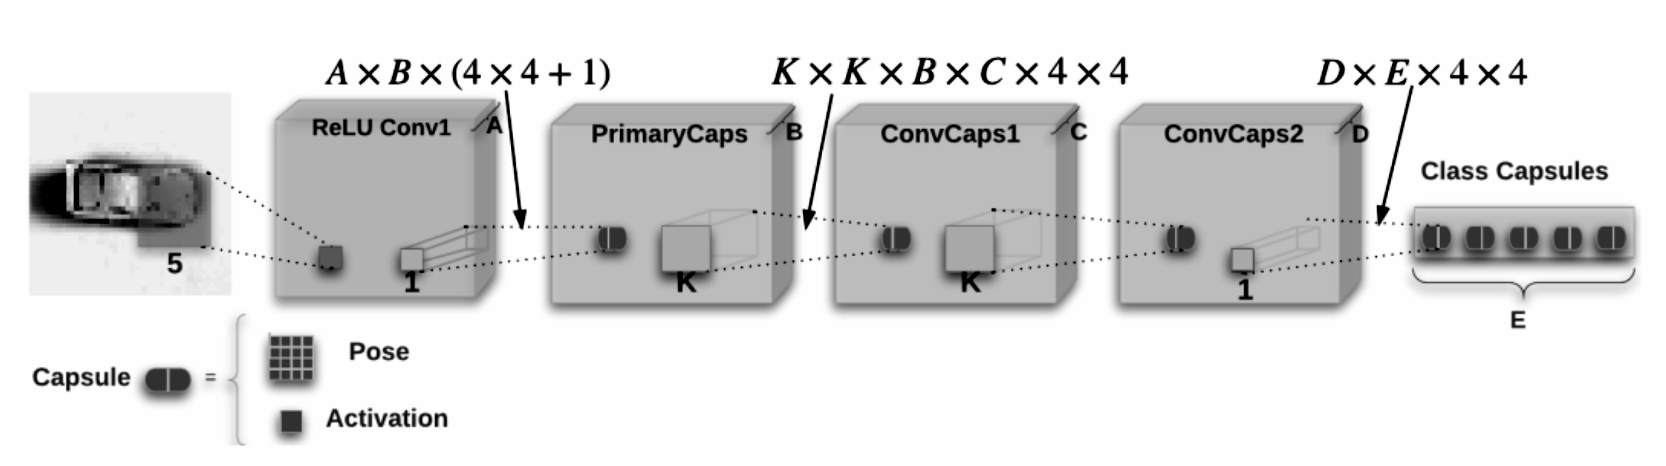
\includegraphics[width=1\textwidth]{images/caps.png}
\caption{Capsule Network}
\end{figure}
The key features of this breakthrough are Layer based Squashing and Dynamic Routing.
In a typical Convolutional Neural Network, the squashing function is added to each layer of the CNN model. A squashing function compresses the input to one of the ends of a small interval, introducing nonlinearity to the neural network and enables the network to be effective. Whereas, in a Capsule network, the squashing function is applied to the vector output of each capsule.\par\bigskip
Instead of applying non-linearity to each neuron, the squashing function applies squashing to a group of neurons i.e the capsule. To be more precise, it applies nonlinearity to the vector output of each capsule. The squashing function also tries to squash the vector output to zero if it is a small vector. If the vector is too long, the function tries to limit the output vector to 1.\par\bigskip
Dynamic routing algorithm in CapsNet replaces the scalar-output feature detectors of the CNN with the vector-output capsules. Also, the max pooling feature in CNNs, which led to positional invariance, is replaced with ‘routing by agreement’. The algorithm ensures that when they forward propagate the data, it goes to the next most relevant capsule in the layer above. Although dynamic routing adds an extra computational cost to the capsule network, it has been proved to be advantageous to the network by making it more scalable and adaptable.

\par
\chapter{Objective}\label{ch:objective}
\epigraph{\textit{\Large “Any A.I. smart enough to pass a Turing test is smart enough to know to fail it.”}}{\textit{ \large Ian McDonald,\\ River of Gods}}
The broad objective is to use the existing Generative Adversarial Networks technologies to aid in the generation of human faces such that the GAN generated images is indistinguishable from the images of the real people used to train the network, i.e fake images should look very much real. This would be then extended to completion of faces, ie. reconstruction of facial features given a partial face.\par\bigskip
The internal specific objective would be to achieve the above said objectives using a ground breaking technology released in fall 2017, the Capsule Nets. The existing latest state-of-the-art GAN architectures use Convolution Neural Networks in their Generators and Discriminators. The CNNs are said to have the drawbacks as mentioned before, where they cannot understand orientation and spatial relationships unless they are extensively trained with all possible images. This major drawback is handled by Capsule Networks.
\par\bigskip
Using the CapsNet architecture into the Generator/Discriminator could improve these Adversarial Networks quite drastically. This mating of the revolutionary Generative Adversarial Networks along with the ground-breaking Capsule Networks, resulting in “Capsule Net GANs” is the overarching objective.

\par
{\chapter{Scope}\label{ch:scope}}
\epigraph{\textit{\Large “By far the greatest danger of Artificial Intelligence is that people conclude too early that they understand it.”}}{\textit{ \large Eliezer Yudkowsky,\\ Machine Intelligence Research Institute}}
Generative Adversarial Networks are one of the hottest topics in Deep Learning right now. The applications of GANs are far ranging and immense. Creating Infographics from text, creating animations for rapid development of marketing content, generating website designs are to name a few. Our focus in this project is to implement a way to complete images of faces by generating the missing pieces using a GAN. 

\par\bigskip
This particular implementation of the technology would be immensely useful in a variety of circumstances. A few straightforward applications include face sketching of suspects in a crime using eye witness accounts, super resolution of CCTV camera footage to enhance faces, filling in of old degraded color photos, etc.
\par
\chapter{Methodology}\label{ch:methodology}
\begin{figure}[H]
\centering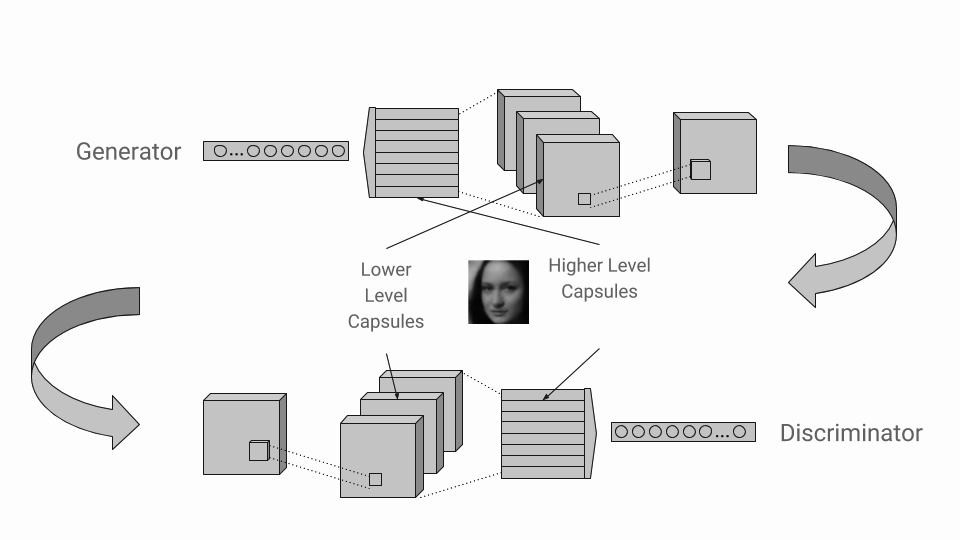
\includegraphics[width=1\textwidth]{images/methodology.png}
\caption{Proposed architecture}
\end{figure}
\par
\chapter{Technology}\label{ch:technology}
\epigraph{\textit{\Large “I think, therefore I am”}}{\textit{ \large René Descartes,\\ French philosopher and scientist}}
\begin{itemize}
	\item\textbf{Adversarial Training:} Two models undergoing training simultaneously by competing against each other. The output of each model acts as an adversary for the other to improve upon.
	\item\textbf{Generative Model:} Any model capable of generating completely new realistic data of a class.
	\item\textbf{Discriminative Model:} Here, as a Discriminator, a model which is capable of distinguishing between actual ground truth from the true distribution and generated information from a model.
	\item\textbf{Gradient Descent:} A method of optimizing an objective function using a first-order iterative approach to find a local minimum.
	\item\textbf{Gaussian Model:} A model that fits the data in the shape of a Gaussian function, identified by a characteristic "bell curve". CapsNet uses this to find agreeing probability outputs of the "capsules".
	\item\textbf{TensorFlow:} An open source software library for numerical computation using data flow graphs. It was originally developed by the Google Brain Team within Google's Machine Intelligence research organization for machine learning and deep neural networks research.

\end{itemize}

\textbf{\Large Other essentials:}

\begin{itemize}
	\item\textbf{CPU:} 3GHz quad core, x86-64 architecture (or)
	\item\textbf{GPU:} NVIDIA or any other TensorFlow supported GPU, CUDA or cuDNN
	\item\textbf{Python:} 2.7 or 3.4 and above
\end{itemize}

\par
\chapter{Conclusion}\label{ch:conclusion}
\epigraph{\textit{\Large “A year spent in artificial intelligence is enough to make one believe in God”}}{\textit{ \large Alan Perlis,\\ First Turning award recepient}}
During the course of this project, we wish to replicate the results of the existing state-of-the-art in Generative Models. Using this as a stepping stone, we would like to incorporate a hitherto unexplored option in CapsNet for Generative Models. Our motivating assumption is that CapsNet would provide a performance improvement.We base this on the idea that it is more capable of understanding the variances in objects. This in turn should lead to lower data requirements during training of the model and consequently lower power consumption. 

\par\bigskip We wish to provide a comparison between our novel CapsNet-based approach and other implementations of GAN for the same task. We would like to implement a proof of concept by developing a application to complete incomplete images of human faces. This could later on be used in enhancement of hazy CCTV footage to identify individuals, which would be immensely helpful to law enforcement personnel.

\vspace{200px}
\centering
\textbf{Head of Department}
\vspace{50px}
\flushleft\textbf{Project Guide}\hfill\textbf{Project Coordinator}
\par\clearpage
\bibliography{ref}{}
\bibliographystyle{plainyr-rev}
\par
\end{document}
